\documentclass{article}
\usepackage{tikz, comment}
\usepackage{pifont}
\usepackage{fontspec}
\usetikzlibrary{arrows, decorations.markings, decorations.pathreplacing}
\begin{comment}
:Title: Not defined yet
:Tags: terms;system;symmetry;symmetric;sector;respect;positive
:Author: Prof.Hu Ji-shan, HKUST
:Slug: No name yet

Description Here.........
\end{comment}
\begin{document}\centering

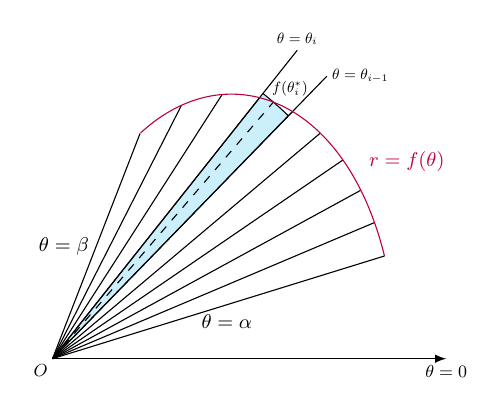
\begin{tikzpicture}[>=latex,xscale=.5*1, yscale=.5*1][font=\sf\small]

\draw[->] (0, 0) -- (10, 0)node[below, scale=0.7] {$\theta=0$};

\node[scale=0.7] at (-0.3/1, -0.3/1) {$O$};

\node[below, xshift=3, scale=0.8] at ({4*((cos(0.3 r)-1.2)^3-0.4*(cos(0.3 r))+1.5)*cos(0.3 r)}, {4*((cos(0.3 r)-1.2)^3-0.4*(cos(0.3 r))+1.5)*sin(0.3 r)}) {$\theta=\alpha$};
\node[left, xshift=0, scale=0.8] at ({4*((cos(1.2 r)-1.2)^3-0.4*(cos(1.2 r))+1.5)*cos(1.2 r)}, {4*((cos(1.2 r)-1.2)^3-0.4*(cos(1.2 r))+1.5)*sin(1.2 r)}) {$\theta=\beta$};

\draw[white, fill=cyan!20, samples=100, smooth, domain= 0.8:0.9, variable=\t]
plot ({8.59882*cos(\t r)}, {8.59882*sin(\t r)}) --(0,0);

\draw[samples=100, smooth, domain= 0.8:0.9, variable=\t]
plot ({8.59882*cos(\t r)}, {8.59882*sin(\t r)});

\draw[dashed] (0, 0)--
({8*((cos((0.3+0.1*(6.6-1)) r)-1.2)^3-0.4*(cos((0.3+0.1*(6.6-1)) r))+1.5)*cos((0.3+0.1*(6.6-1)) r)}, {8*((cos((0.3+0.1*(6.6-1)) r)-1.2)^3-0.4*(cos((0.3+0.1*(6.6-1)) r))+1.5)*sin((0.3+0.1*(6.6-1)) r)})
node[above, xshift=6, scale=0.6] {$f(\theta_i^*)$};

\draw[] (0, 0)--
({10*cos((0.3+0.1*(6-1)) r)}, {10*sin((0.3+0.1*(6-1)) r)}) node[right, scale= 0.6] {$\theta = \theta_{i-1}$};
\draw[] (0, 0)--
({10*cos((0.3+0.1*(7-1)) r)}, {10*sin((0.3+0.1*(7-1)) r)}) node[above, scale= 0.6] {$\theta = \theta_{i}$};

\foreach \x in {1,2,...,10}
\draw[black, fill=cyan!20][fill opacity=1] (0, 0)--
({8*((cos((0.3+0.1*(\x-1)) r)-1.2)^3-0.4*(cos((0.3+0.1*(\x-1)) r))+1.5)*cos((0.3+0.1*(\x-1)) r)}, {8*((cos((0.3+0.1*(\x-1)) r)-1.2)^3-0.4*(cos((0.3+0.1*(\x-1)) r))+1.5)*sin((0.3+0.1*(\x-1)) r)});

\draw[purple, samples=100, smooth, domain= 0.3:1.2, variable=\t]
plot ({8*((cos(\t r)-1.2)^3-0.4*(cos(\t r))+1.5)*cos(\t r)}, {8*((cos(\t r)-1.2)^3-0.4*(cos(\t r))+1.5)*sin(\t r)}) ;

\node[purple, scale=0.8] at (9, 5) {$r = f(\theta)$};

\end{tikzpicture}
\end{document}